\documentclass[../../Main.tex]{subfiles}

\begin{document}
    \begin{figure}[hbt!]
        \centerline{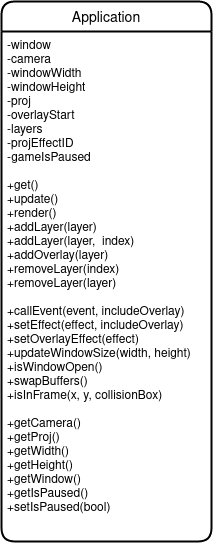
\includegraphics[scale=0.5]{img/Classes/Application.png}}
        \caption{Application class (singleton)}
        \label{fig}
    \end{figure}
    \begin{center}
        Variables
        \addvbuffer[12pt 8pt]{\begin{tabular}{ | m{0.45\textwidth} | m{0.45\textwidth} | }
            \hline
            \textbf{Variable Name} & \textbf{\textbf{Description}} \\
            \hline
            window & Stores the application window itself \\
            \hline
            camera & Stores the camera that effects the non-overlay layers \\
            \hline
            windowWidth & Stores the width of the window \\
            \hline
            windowHeight & Stores the height of the window \\
            \hline
            proj & Stores the projection map matrix for the window \\
            \hline
            overlayStart & Stores the position at which the overlay layers start in the layer stack \\
            \hline
            layers & Stores the layer stack \\
            \hline
            projEffectID & Stores the ID of the projection effect for all the layers \\
            \hline
            gameIsPaused & Stores whether the game is paused or not \\
            \hline
        \end{tabular}}

        \clearpage
        Functions
        \begin{tabular}{ | m{0.15\textwidth} | m{0.35\textwidth}| m{0.4\textwidth} | }
            \hline
            \textbf{Function Name} & \textbf{Parameters} & \textbf{Description} \\
            \hline
            get & & Returns the single instance of the Application \\
            \hline
            update & & Calls the update function on all the layers \\
            \hline
            render & & Calls the render function on all the layers \\
            \hline
            addLayer & Layer you wish to add & Adds a layer to the stack (under the overlays)\\
            \hline
            addOverlay & Overlay (as a layer) you wish to add & Adds a layer to the stack on top of all the other layers \\
            \hline
            removeLayer & Either the index of the layer or the layer you wish to remove & Removes a layer from the stack \\
            \hline
            callEvent & Event and boolean to tell it whether to include the overlay & Calls the event on every layer until one of them uses it \\
            \hline
            setEffect & Effect and boolean to tell it whether to include the overlay & Sends the effect to every layer until one of them uses it \\
            \hline
            setOverlay & An effect to send & Sends an effect through only the overlays until one of them uses it \\
            \hline
            updateWindowSize & The new width and height of the window & Updates the window size stored in the Application \\
            \hline
            isWindowOpen & & Returns whether the application is open or not \\
            \hline
            swapBuffers & & Swaps the buffers of the application (for rendering) \\
            \hline
            isInFrame & x and y of the object and the collision box of the object & Acts as a go between for the camera's isInFrame function \\
            \hline
            getCamera & & Returns the camera used for the non-overlay layers \\
            \hline
            getProj & & Returns the projection map for the application window \\
            \hline
            getWidth & & Returns the width of the application window \\
            \hline
            getHeight & & Returns the height of the application window \\
            \hline
            getWindow & & Returns the openGL window \\
            \hline
            getIsPaused & & Returns whether the game is paused or not (preventing the non-overlay functions from being updated) \\
            \hline
            setIsPaused & boolean that the isPaused variable is set to & Sets the isPaused variable \\
            \hline
        \end{tabular}
    \end{center}
\end{document}